\chapter{Installation and Configuration}
\partlabel{PART IV --- PRACTICAL USER GUIDE}
\section{Start the existing local stack}
\begin{enumerate}
\item Install Docker Engine with Compose v2. Native development additionally uses the repository's npm workspace dependencies; Docker builds use Node 24. RAG/ML builds need disk space for Python/model packages and initial internet access. Core inference needs OpenAI connectivity and an operator-provided key.
\item From the repository root, create \texttt{.env} only if absent. Set a strong \texttt{DB\_PASSWORD} locally. Preserve the password of an existing initialized database volume; changing the file alone does not update PostgreSQL's stored password.
\item Build/start the three-service application, then check its health.
\end{enumerate}
\begin{lstlisting}[language=bash]
test -e .env || cp .env.example .env
# Edit .env locally; keep all existing confidential entries.
chmod 600 .env
docker compose up --build -d --wait
curl http://127.0.0.1:8000/api/health
\end{lstlisting}
Open \url{http://localhost:8080}. The database is private; its \texttt{message-data} volume persists across ordinary restarts. Avoid deleting volumes. If external containers are already connected, retain the MCP overlay on subsequent core Compose commands (Chapter 12).
\section{Save the model connection}
\begin{minipage}[t]{.65\linewidth}
\begin{enumerate}
\item Expand \textbf{LLM}; company is currently OpenAI.
\item Enter a replacement API key and press \textbf{Save API key}. Input clears after submission. There is no reveal control.
\item Choose a model from the authenticated catalog; \textbf{Refresh} reloads it.
\item Choose \textbf{Instant}, \textbf{Medium} or \textbf{High} thinking, then \textbf{Save settings}.
\item Send a small ordinary message to confirm compatibility. Discovery alone does not prove text/structured-output support.
\end{enumerate}
For context-capacity overrides or cost limits, edit the root environment settings described in \path{docs/OPERATIONS.md} and \path{docs/TASK_EXECUTION.md}. Restart core after static worker/policy changes. Do not place tokens in frontend build variables.
\end{minipage}\hfill
\begin{minipage}[t]{.29\linewidth}\vspace{0pt}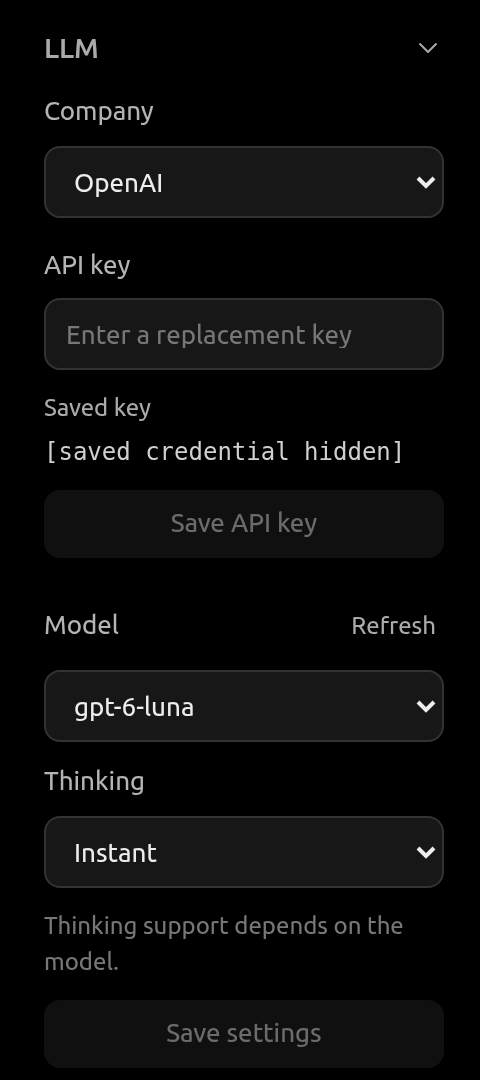
\includegraphics[width=\linewidth]{figures/ui-llm-panel.png}\captionof{figure}{Live LLM panel. Saved-key text hidden for publication.}\end{minipage}
\note{First-use checks}{New chat opens the existing composer. \textbf{+} stores/downloads ordinary attachments; it does not index them. Enter sends and Shift+Enter adds a line. Use \textbf{RAG → Documents} for searchable manual uploads.}
\source{\path{README.md}; \path{docker-compose.yml}; \path{.env.example}; \path{core/src/config/environment.ts}; \path{ui/src/components/llm/llm-settings.tsx}.}
